\documentclass{article}
\usepackage{graphicx}
\usepackage{amsmath}
\title{\textbf{homework-01}}
\author{our group name here}
\date{\today}

\begin{document}
\maketitle

\section{Broken Chessboard and Jumping With Coins}
\subsection{Tiling a Damaged Checkerboard}

\begin{flushleft}
\textbf{Exercise 1.1.} \\
Firstly, we color the chessboard in black and white.\\
\begin{center}
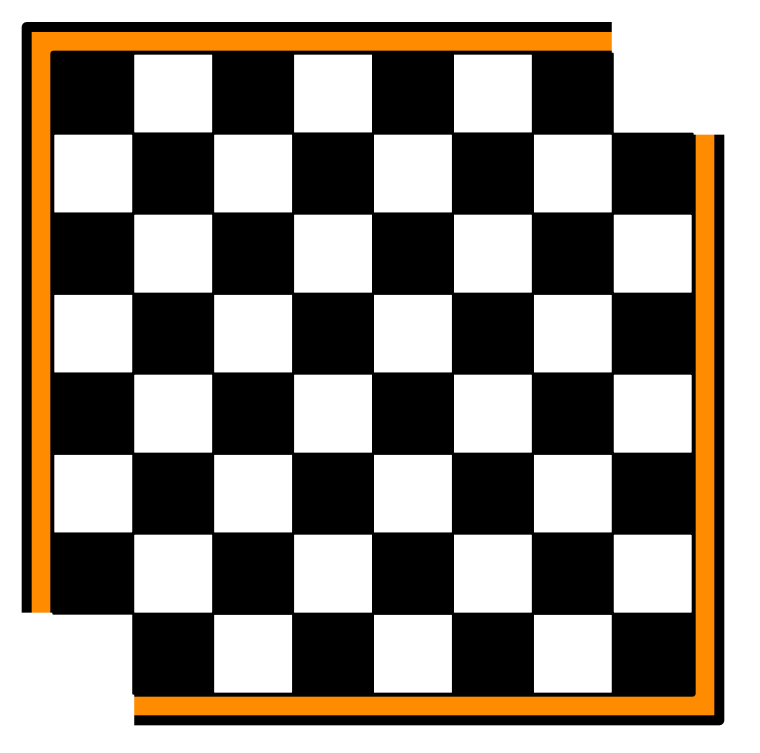
\includegraphics[scale=0.3]{1_1_1.png}
\end{center}
So now, we have 32 black squares and 30 white squares.\\
And if we put a tile in this chessboard, it will cover exactly a black square and a white squre, no matter how we put it.\\
So if we continue put tiles on it, we will have two black squares left in the end.\\
\begin{center}
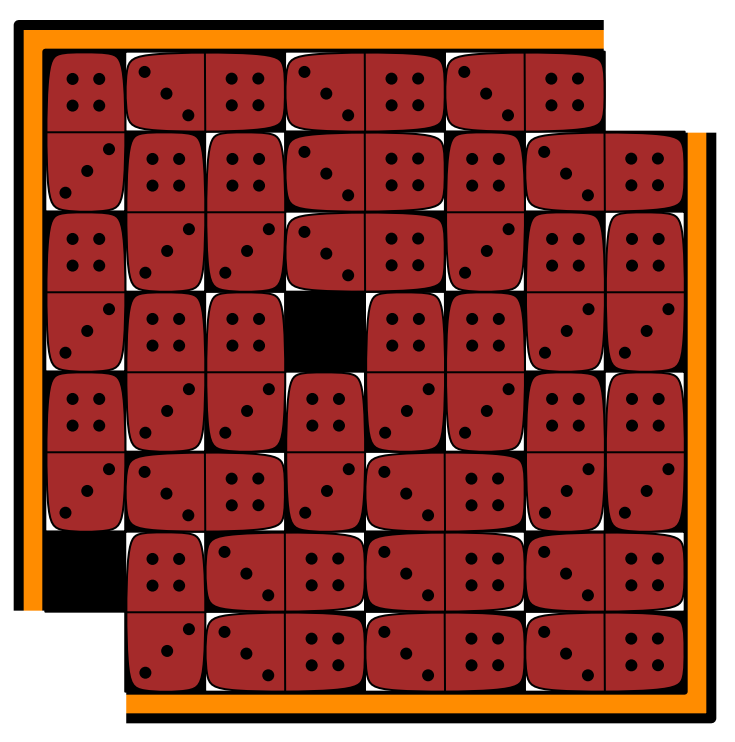
\includegraphics[scale=0.3]{1_1_2.png}
\end{center}
It means that whatever we do we will always get stuck because there are always two more black squares than white squares.\\
So it is obvious that we cannot tile this damaged chessboard.\\

\textbf{Exercise 1.2.} \\
...

\end{flushleft}
\subsection{Jumping with Coins}

\begin{flushleft}
\textbf{Exercise 1.3.} \\
Obviously, we have only two coins, so that each of them can only jump over the other one.
In this case, the distance between the two coins will never change. So we cannot increase the 
distance between the two coins.

\textbf{Exercise 1.4.} \\
...

\textbf{Exercise 1.5.} \\
A coin is at a position $(x,y)\in\mathbf{R}^2$ .\\
we assume that in the beginning the positions are (0,0),(0,1),(1,0),(1,1).\\
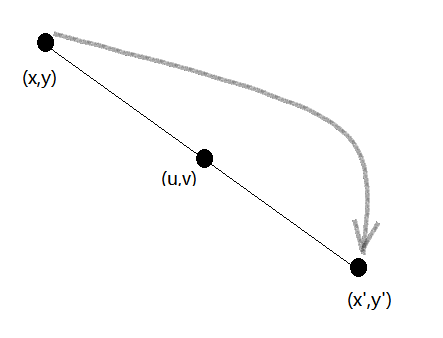
\includegraphics[scale=1]{1_5_1.png}\\
$(u,v)+(u,v)-(x,y)=(2u-x,2v-y)$\\
If $(u,v),(x,y)\in\mathbf{Z}^2$ , then $(2u-x,2v-y)\in\mathbf{Z}^2$.\\
Thus the coins will always be on an integer position.
Now let (x,y) be the position of a coin,\\
if $(x,y)\in\mathbf{Z}^2$, we can say coin is
$
\left\{\begin{array}{ll}
white & \textrm{while x+y is odd}\\
black & \textrm{while x+y is even}
\end{array} \right.
$
.\\
So, now the color of (x,y) is $(x+y)\mod2$, the color of (2u-x,2u-y) is $[(2u-x)+(2v-y)]\mod2=(x+y)\mod2$
,they are on the same color square.\\
Considering that, we put four coins on a chessboard like this:
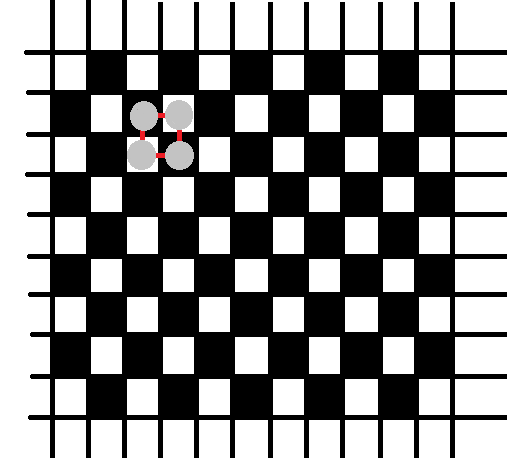
\includegraphics[scale=0.8]{1_5_2.png}\\
We can see there are two coins on white square and two on black square.\\
And if the side length of coin square becomes 2, it will look like this:
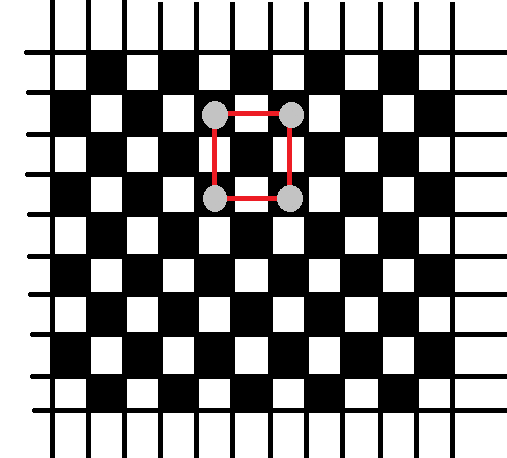
\includegraphics[scale=0.8]{1_5_3.png}\\
In this situation, all coins are on white (or black) square. 
But we have already proved that every coin's color will not change, so this pattern can never be achieved.

\textbf{Exercise 1.6.} \\
...

\textbf{Exercise 1.7.} \\
If we can turn the origin square into a pattern, we can also turn this pattern
into a square whose side length is 1 by undoing every step reversely. \\
So now we assume that we have a larger square of side length $a(a>1)$ 
and the positions are $(0,0),(0,a),(a,a),(a,0).$\\
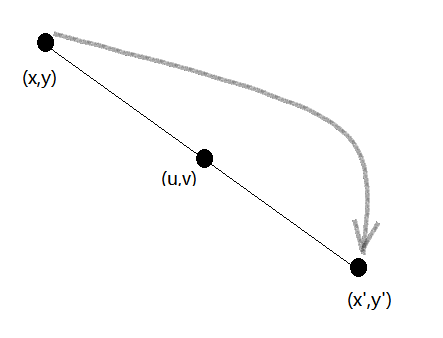
\includegraphics[scale=1]{1_5_1.png}\\
$(u,v)+(u,v)-(x,y)=(2u-x,2v-y)$\\
If $(u,v),(x,y)\in\mathbf{Z}^2$ , then $(2u-x,2v-y)\in\mathbf{Z}^2$.\\
Thus the coins will always be on an integer position.
Now let (x,y) be the position of a coin, if $x\mod a=0$ and $u\mod a=0$ then $(2u-x)\mod a=0$
and so it is with vertical ordinate. It means that whatever we do, the distance between any two
coins will be at least $a$ (Two coins cannot be at the same position, which is proved by us in 
Exercise 1.6.). In this situation, we will never get a smaller square. Meanwhile, it proves that 
we can never get a larger square.

\textbf{Exercise 1.8.} \\
...

\end{flushleft}
\section{Exclusion-Inclusion}
\subsection{Sets}

\begin{flushleft}
\textbf{Exercise 2.1.} \\
...

\textbf{Exercise 2.2.} \\
...

\textbf{Exercise 2.3.} \\
...

\end{flushleft}
\section{Feasible Intersection Patterns}

\begin{flushleft}
\textbf{Exercise 3.1.} \\
...

\textbf{Exercise 3.2.} \\
...

\textbf{Exercise 3.3.} \\
...
\end{flushleft}
\end{document}